\documentclass[10pt,a4paper]{article}
\usepackage[utf8]{inputenc}
\usepackage{amsmath}
\usepackage{amsfonts}
\usepackage{amssymb}
\usepackage{graphicx}
\usepackage{fancyhdr}
\pagestyle{fancy}
\fancyhf{}
\rhead{Justin Anguiano 2700353}
\lhead{PHSX 815 Final Project}
\begin{document}

\section{}
\subsection{}
Minimizing the equation 
\begin{equation}
f(x,y) = 100(y-x^2)^ + (1-x)^2
\end{equation}
using the NelderMead simplex algorithm with the initial simplex vertices $ (x,y) : {(-1.2,1.0), (-2,1) ,(1,0)}$. The minimum found is points $(1,1)$ with a function value $8.04756e-15$ compared to the actual minimum $f(1,1) = 0$.

\subsection{}
Using the equation 
\begin{equation}
		f(x,y) = g(x,y)h(x,y)
\end{equation}
where
\begin{equation}
	g(x,y) = 1 + (x+y+1)^2(19-14x+3x^2 -14y+6xy+3y^2)
\end{equation}
and
\begin{equation}
	h(x,y) = 30 + (2x-3y)^2(18-32x+12x^2+48y-36xy+27y^2)
\end{equation}
To find four local minima the NelderMead simplex algorithm was used again with initial simplex vertice guesses based on approximations near the minima from visualization of the function.

\begin{tabular}{|c|c|}
\hline 
Minimum (x,y) & f(x,y) \\ 
\hline 
(-0.499202, -0.499202) &  32.6845 \\ 
\hline 
(1, -0.334639) & 94.6492
 \\ 
\hline 
(1.8, 0.2) & 84 \\ 
\hline 
 (-0.335, -0.670001) & 33.5259 \\ 
\hline 
\end{tabular} 

\section{}
Analyzing the data from measurements2.dat with parameters $(x,y,\sigma)$ by fitting with the 4-parameter nonlinear model
\begin{equation}
	f(x) = V_0 + Asin(\omega x - \phi)
\end{equation}
and minimizing the $\chi^2$ using the NelderMead simplex algorthim
\begin{equation}
	\chi^2 = \sum_{i=1}^{n} (\frac{f(x_i) - y_i}{\sigma_i})^2
\end{equation}
The resulting optimal parameters $(V_0, A, \omega, \phi)$ are $ (3.14139, 0.119546, 9.54645, 9.21187)$ with a $\chi^2$ value of $82.9194$

\section{}
For solving the 130 city traveling salesman problem, the genetic algorithm was used. The implementation uses an arbitrary population size with initially randomized solutions to the problem.  The population is randomly sampled from an arbitrary sample size, the two lowest cost solutions are combined to form a child in the next generation of the population. This process is continues until the child generation is of equal size to the preceding parent population.  The parent solutions are combined by selecting a random continuous subset of city traversals from the first parent and placing them in the same order and location in the child. Then the non-repeating elements from the second parent are placed into the child. The breeding process is illustrated below. \\
Parents
\begin{figure}[h]
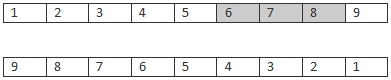
\includegraphics[width=7cm]{crossover_parents.jpg}
\end{figure}\\
Child
\begin{figure}[h]
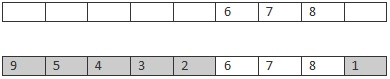
\includegraphics[width=7cm]{crossover_children.jpg}
\scriptsize source: http://www.theprojectspot.com/tutorial-post/applying-a-genetic-algorithm-to-the-travelling-salesman-problem/5
\end{figure}
\\
Each crossover is also subject to mutations with an arbitrary rate of mutation. The mutation swaps two random cities in the trip solution.\\
When the algorithm is run with a population size of 75 and sample size of 20, the consistently achievable lowest cost solutions hover around 39000, but the 1 time optimal solution generated was 37602.8 after 53 generations.





\end{document}